In 1996, the first widely deployed SIMD (Single Instruction, Multiple Data according to Flynn’s taxonomy) instruction set was MMX extensions on top of the x86 architecture. Many SIMD instruction set extensions have since followed both on Intel architectures and more broadly across the industry. A CPU core carries out its job by executing instructions, and the specific instructions that a core knows how to execute are defined by the instruction set (e.g., x86, x86\_64, AltiVec, NEON) and instruction set extensions (e.g., SSE, AVX, AVX-512) that it implements. Many of the operations added by instruction set extensions are focused on SIMD instructions.\par

SIMD instructions allow multiple calculations to be carried out simultaneously on a single core by using a register and hardware that is bigger than the fundamental unit of data being processed. Using 512-bit registers, we can perform eight 64-bit calculations with a single machine instruction.\par

\hspace*{\fill} \par %插入空行
Figure 16-2. SIMD execution in a CPU hardware thread
\begin{center}
	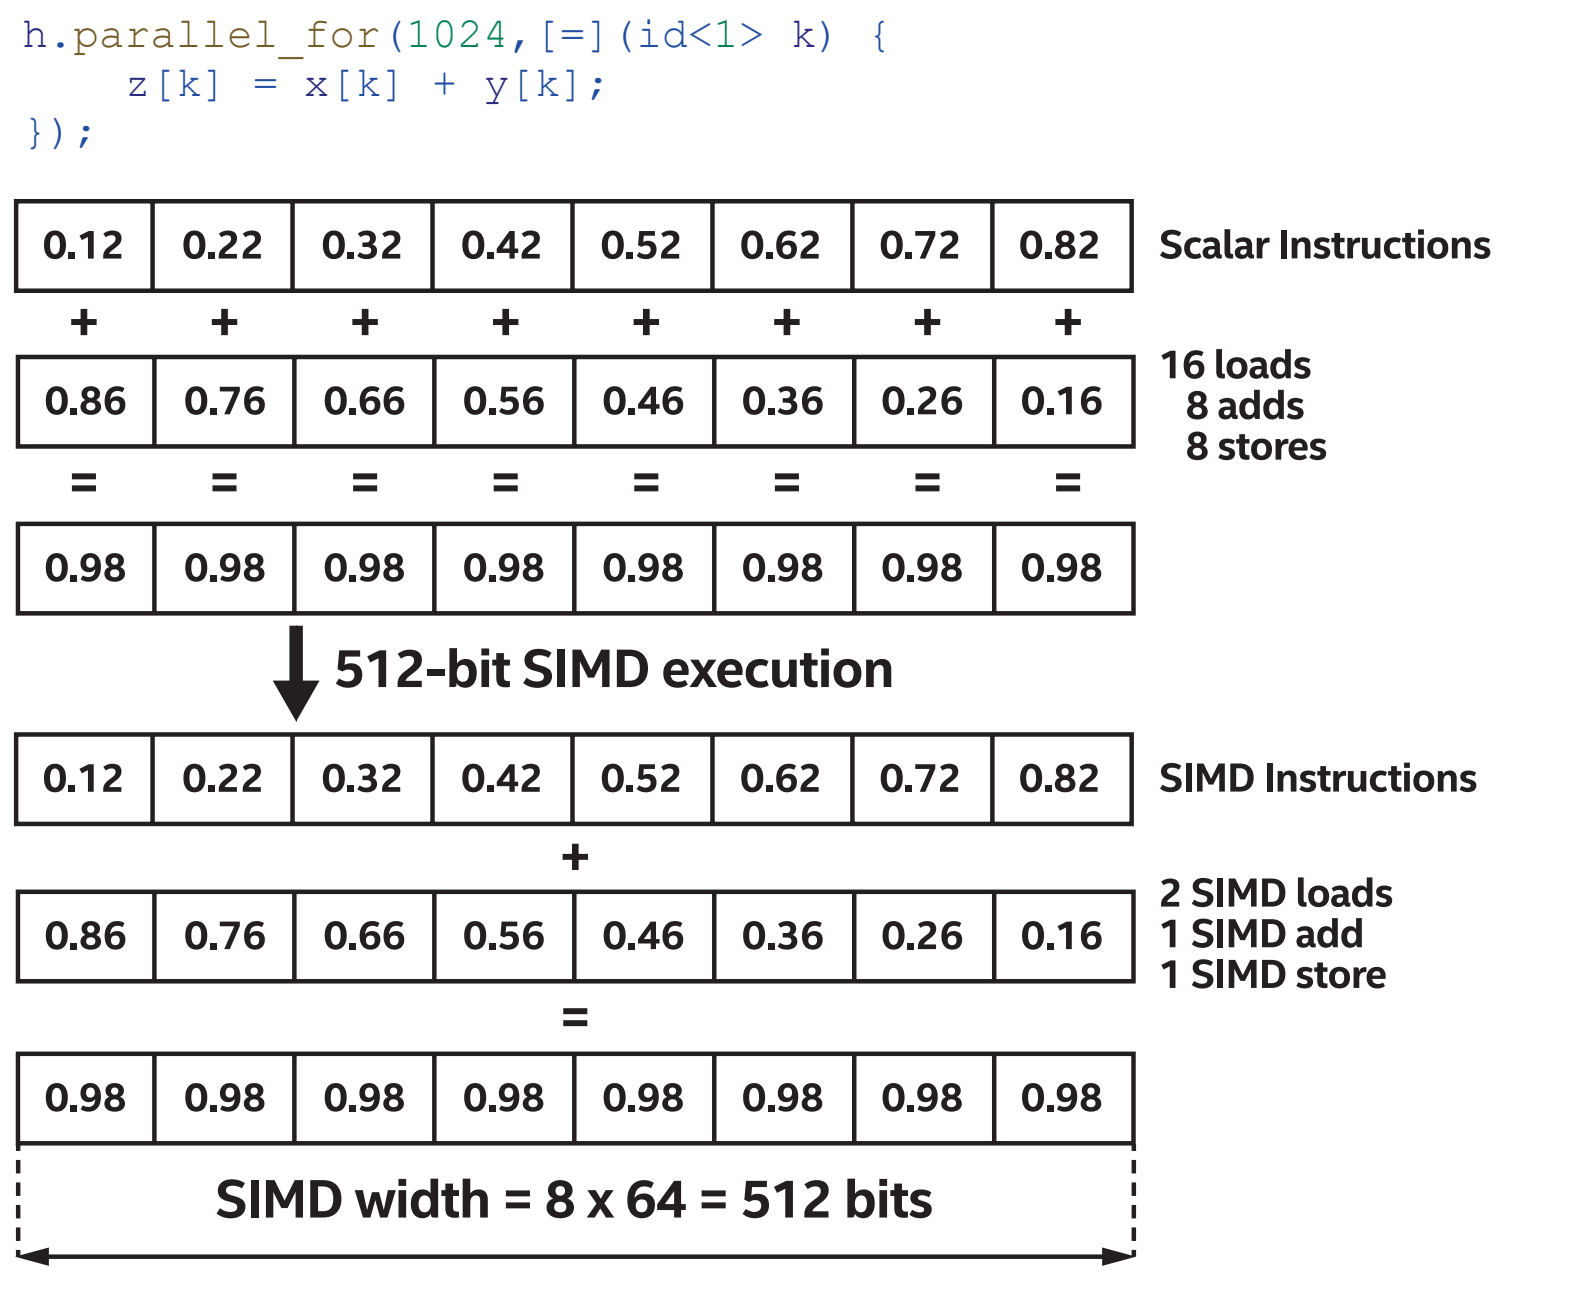
\includegraphics[width=1.0\textwidth]{content/chapter-16/images/3}
\end{center}

This example shown in Figure 16-2 could give us up to an eight times speed-up. In reality, it is likely to be somewhat curtailed as a portion of the eight times speed-up serves to remove one bottleneck and expose the next, such as memory throughput. In general, the performance benefit of using SIMD varies depending on the specific scenario, and in a few cases, it can even perform worse than simpler non-SIMD equivalent code. That said, considerable gains are achievable on today’s processors when we know when and how to apply (or have the compiler apply) SIMD. As with all performance optimizations, programmers should measure the gains on a typical target machine before putting it into production. There are more details on expected performance gains in following sections of this chapter.\par

The cc-NUMA CPU architecture with SIMD units forms the foundation of a multicore processor, which can exploit a wide spectrum of parallelism starting from instruction-level parallelism in five different ways as shown in Figure 16-3.\par

\hspace*{\fill} \par %插入空行
Figure 16-3. Five ways for executing instructions in parallel
\begin{center}
	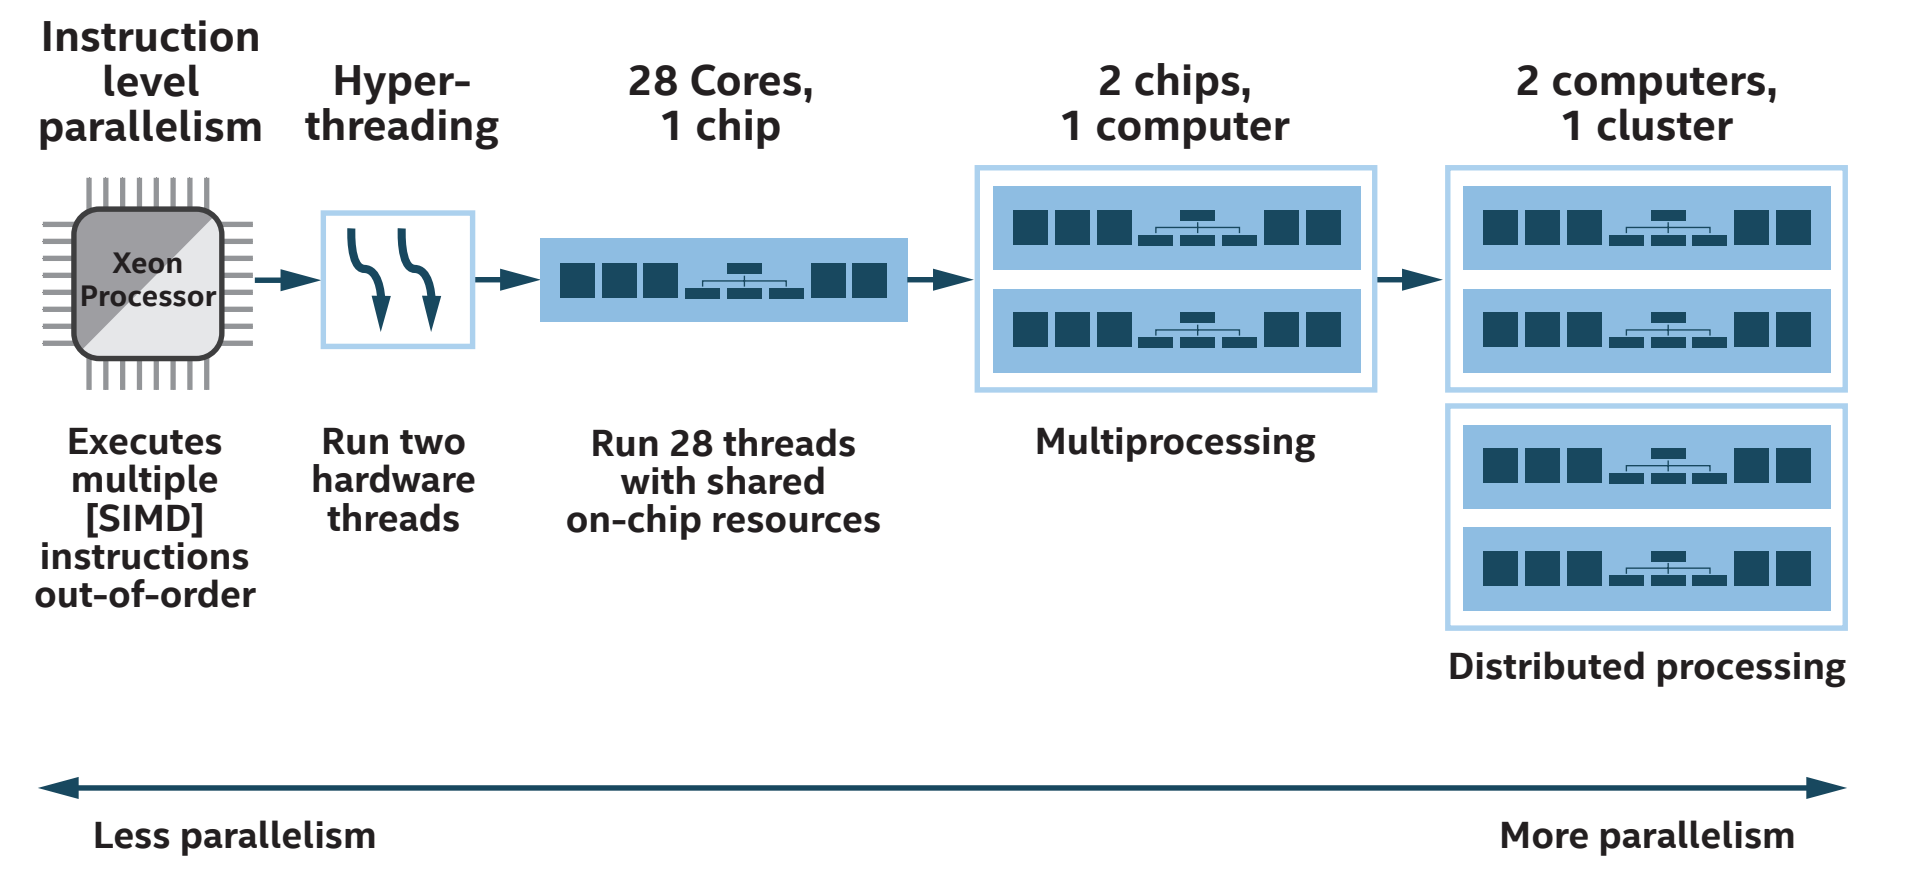
\includegraphics[width=1.0\textwidth]{content/chapter-16/images/4}
\end{center}

In Figure 16-3, instruction-level parallelism can be achieved through both out-of-order execution of scalar instructions and SIMD (Single Instruction, Multiple Data) data parallelism within a single thread. Threadlevel parallelism can be achieved through executing multiple threads on the same core or on multiple cores at different scales. More specifically, thread-level parallelism can be exposed from the following:\par

\begin{itemize}
	\item Modern CPU architectures allow one core to execute the instructions of two or more threads simultaneously.
	\item Multicore architectures that contain two or more brains within each processor. The operating system perceives each of its execution cores as a discrete processor, with all of the associated execution resources.
	\item Multiprocessing at the processor (chip) level, which can be accomplished by executing completely separate threads of code. As a result, the processor can have one thread running from an application and another thread running from an operating system, or it can have parallel threads running from within a single application.
	\item Distributed processing, which can be accomplished by executing processes consisting of multiple threads on a cluster of computers, which typically communicate through message passing frameworks.
\end{itemize}

In order to fully utilize a multicore processor resource, the software must be written in a way that spreads its workload across multiple cores. This approach is called exploiting thread-level parallelism or simply threading.\par

As multiprocessor computers and processors with hyper-threading (HT) technology and multicore technology become more and more common, it is important to use parallel processing techniques as standard practice to increase performance. Later sections of this chapter will introduce the coding methods and performance-tuning techniques within DPC++ that allow us to achieve peak performance on multicore CPUs.\par

Like other parallel processing hardware (e.g., GPUs), it is important to give the CPU a sufficiently large set of data elements to process. To demonstrate the importance of exploiting multilevel parallelism to handle a large set of data, consider a simple C++ STREAM Triad program, as shown in Figure 16-4.\par

\begin{tcolorbox}[colback=blue!5!white,colframe=blue!75!black, title=A NOTE ABOUT STREAM TRIAD WORKLOAD]
The STREAM Triad workload (www.cs.virginia.edu/stream) is an important and popular benchmark workload that CPU vendors use to demonstrate highly tuned performance. We use the STREAM Triad kernel to demonstrate code generation of a parallel kernel and the way that it is scheduled to achieve significantly improved performance through the techniques described in this chapter. The STREAM Triad is a relatively simple workload, but is sufficient to show many of the optimizations in an understandable way.
\end{tcolorbox}

\begin{tcolorbox}[colback=blue!5!white,colframe=blue!75!black, title=USE VENDOR-PROVIDED LIBRARIES!]
When a vendor provides a library implementation of a function, it is almost always beneficial to use it rather than re-implementing the function as a parallel kernel!
\end{tcolorbox}

\hspace*{\fill} \par %插入空行
Figure 16-4. STREAM Triad C++ loop
\begin{lstlisting}[caption={}]
// C++ STREAM Triad workload
// __restrict is used to denote no memory aliasing among arguments 
template <typename T>
double triad(T* __restrict VA, T* __restrict VB, 
			 T* __restrict VC, size_t array_size, const T scalar) {
	double ts = timer_start()
	for (size_t id = 0; id < array_size; id++) {
		VC[id] = VA[id] + scalar * VB[id];
	}
	double te = timer_end();
	return (te – ts); 
}
\end{lstlisting}

The STREAM Triad loop may be trivially executed on a CPU using a single CPU core for serial execution. A good C++ compiler will perform loop vectorization to generate SIMD code for the CPU that has SIMD hardware to exploit instruction-level SIMD parallelism. For example, for an Intel Xeon processor with AVX-512 support, the Intel C++ compiler generates SIMD code as shown in Figure 16-5. Critically, the compiler’s transformation of the code reduced the number of loop iterations at execution time, by doing more work (SIMD width and also unrolled iterations) per loop iteration at runtime!\par

\hspace*{\fill} \par %插入空行
Figure 16-5. AVX-512 code for STREAM Triad C++ loop
\begin{lstlisting}[caption={}]
// STREAM Triad: SIMD code generated by the compiler, where zmm0, zmm1 
// and zmm2 are SIMD vector registers. The vectorized loop is unrolled by 4
// to leverage the out-of-execution of instructions from Xeon CPU and to
// hide memory load and store latency 

# %bb.0: # %entry
vbroadcastsd %xmm0, %zmm0 # broadcast “scalar” to SIMD reg zmm0
movq $-32, %rax
.p2align 4, 0x90
.LBB0_1: # %loop.19
# =>This Loop Header: Depth=1
vmovupd 256(%rdx,%rax,8), %zmm1 # load 8 elements from memory to zmm1 
vfmadd213pd 256(%rsi,%rax,8), %zmm0, %zmm1 # zmm1=(zmm0*zmm1)+mem
# perform SIMD FMA for 8 data elements 
# VC[id:8] = scalar*VB[id:8]+VA[id:8] 
vmovupd %zmm1, 256(%rdi,%rax,8) # store 8-element result to mem from zmm1 
# This SIMD loop body is unrolled by 4
vmovupd 320(%rdx,%rax,8), %zmm1
vfmadd213pd 320(%rsi,%rax,8), %zmm0, %zmm1 # zmm1=(zmm0*zmm1)+mem
vmovupd %zmm1, 320(%rdi,%rax,8)
vmovupd 384(%rdx,%rax,8), %zmm1
vfmadd213pd 384(%rsi,%rax,8), %zmm0, %zmm1 # zmm1=(zmm0*zmm1)+mem
vmovupd %zmm1, 384(%rdi,%rax,8)
vmovupd 448(%rdx,%rax,8), %zmm1
vfmadd213pd 448(%rsi,%rax,8), %zmm0, %zmm1 # zmm1=(zmm0*zmm1)+mem
vmovupd %zmm1, 448(%rdi,%rax,8)
addq $32, %rax
cmpq $134217696, %rax # imm = 0x7FFFFE0
jb .LBB0_1
\end{lstlisting}

As shown in Figure 16-5, the compiler was able to exploit instructionlevel parallelism in two ways. First is through the use of SIMD instructions, exploiting instruction-level data parallelism, in which a single instruction can process eight double-precision data elements simultaneously in parallel (per instruction). Second, the compiler applied loop unrolling to get the out-of-order execution effect of these instructions that have no dependences between them, based on hardware multiway instruction scheduling.\par

If we try to execute this function on a CPU, it will probably run well—not great, though, since it does not utilize any multicore or threading capabilities of the CPU, but good enough for a small array size. If we try to execute this function with a large array size on a CPU, however, it will likely perform very poorly because the single thread will only utilize a single CPU core and will be bottlenecked when it saturates the memory bandwidth of that core.\par

























































